\question
Сапёр Вася получил карту, на которой отображено расположение мин на минном поле. Чтобы обезвредить мины, Васе нужно объединять их проводами в группы по 2, 4 или 8 по особым правилам. Вспомнив знания полученные ещё в университете, Вася заметил, что правила объединение мин совпадают с правилами объединения минтермов на карте Карно. Помоги Васе обезвредить мины. В ответе записать получившуюся функцию в виде МДНФ.

\begin{figure}[h]

\begin{minipage}[h]{0.55\linewidth}
\end{minipage}
\begin{minipage}[h]{0.45\linewidth}
\center{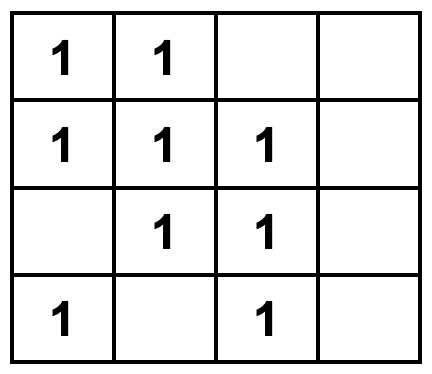
\includegraphics[width=0.7\textwidth]{pic/241.png} }
\end{minipage}
\end{figure}

---------------

Автор -- Никита Салов